\documentclass[letterpaper,12pt]{article}
\usepackage{tabularx} % extra features for tabular environment
\usepackage{amsmath}  % improve math presentation
\usepackage{graphicx} % takes care of graphic including machinery
\usepackage[margin=1in,letterpaper]{geometry} % decreases margins
\usepackage{cite} % takes care of citations
\usepackage[final]{hyperref} % adds hyper links inside the generated pdf file
\hypersetup{
	colorlinks=true,       % false: boxed links; true: colored links
	linkcolor=black,        % color of internal links
	citecolor=blue,        % color of links to bibliography
	filecolor=magenta,     % color of file links
	urlcolor=blue         
}
\usepackage{blindtext}

%%%%%%%%%%%%%%%%%%%%%%%%%%%%%%%%%%%%%%%%%%%%%%%%%%%%%%%%%%%%%%%%%%%%%%%%%%%%%%%%%%%%%%%

% MY PACKAGES

% smart par skip
\usepackage{parskip}

% used to create cute quote 
\usepackage{csquotes}

% fix annoying positioning
\usepackage{float}

% cute tables
\usepackage{booktabs}

% testo intorno a figure
\usepackage{wrapfig, blindtext}

% used to highlight stuff
\usepackage{color,soul}

% MORE MATH
\usepackage{amsfonts}
\usepackage{amsmath}
\usepackage{amssymb}
\usepackage{mathrsfs}

% line breaks in cells
\usepackage{makecell, boldline}

% fix urls in bib
\usepackage{etoolbox}
\appto\UrlBreaks{\do\-}

%%%%%%%%%%%%%%%%%%%%%%%%%%%%%%%%%%%%%%%%%%%%%%%%%%%%%%%%%%%%%%%%%%%%%%%%%%%%%%%%%%%%%%%

% CUSTOM SETTINGS

\setlength\parindent{0pt}

% IMAGES SHORTCUT
\graphicspath{ {./images/} }

% INLINE CODE TEXT
\definecolor{codegray}{gray}{0.9}
\newcommand{\code}[1]{\colorbox{codegray}{\texttt{#1}}}

% CUSTOM LINESPREAD
\linespread{1.05}

% FAST CENTERED IMAGE
\newcommand{\imgc}[3]{\begin{figure}[H] 
  \centering
  \includegraphics[width=#1]{#2}
  \caption{#3}
\end{figure}}

% FIX CAPTION SPACE
\usepackage[font=small,skip=0.25cm]{caption}
\setlength{\belowcaptionskip}{-0.25cm}

% custom line width
\makeatletter
\def\thickhline{%
  \noalign{\ifnum0=`}\fi\hrule \@height \thickarrayrulewidth \futurelet
   \reserved@a\@xthickhline}
\def\@xthickhline{\ifx\reserved@a\thickhline
               \vskip\doublerulesep
               \vskip-\thickarrayrulewidth
             \fi
      \ifnum0=`{\fi}}
\makeatother

% custom citations
\usepackage{cite}

%%%%%%%%%%%%%%%%%%%%%%%%%%%%%%%%%%%%%%%%%%%%%%%%%%%%%%%%%%%%%%%%%%%%%%%%%%%%%%%%%%%%%%%

% CUSTOM PYTHON CODE

\usepackage{listings}
\usepackage{xcolor}

\definecolor{codegreen}{rgb}{0,0.6,0}
\definecolor{codegray}{rgb}{0.5,0.5,0.5}
\definecolor{codepurple}{rgb}{0.58,0,0.82}
\definecolor{backcolour}{rgb}{0.95,0.95,0.92}

\lstdefinestyle{mystyle}{
    backgroundcolor=\color{backcolour},   
    commentstyle=\color{codegreen},
    keywordstyle=\color{magenta},
    numberstyle=\tiny\color{codegray},
    stringstyle=\color{codepurple},
    basicstyle=\ttfamily\footnotesize,
    breakatwhitespace=false,         
    breaklines=true,                 
    captionpos=b,                    
    keepspaces=true,                 
    numbers=left,                    
    numbersep=5pt,                  
    showspaces=false,                
    showstringspaces=false,
    showtabs=false,                  
    tabsize=2
}

\lstset{style=mystyle}

%%%%%%%%%%%%%%%%%%%%%%%%%%%%%%%%%%%%%%%%%%%%%%%%%%%%%%%%%%%%%%%%%%%%%%%%%%%%%%%%%%%%%%%

\begin{document}

\title{\textbf{Network and Practical}}
\author{\textbf{Introduction to ML for Natural Language Processing}\\ \\ Daniele Passabì [221229], Data Science\\}

\date{\textit{\\Multi-class Classification of European Laws in Five Languages\\How do Statistical Models and Recurrent Neural Networks Behave?}}
\maketitle
\thispagestyle{empty}

\begin{figure}[H] 
  \centering
  
\includegraphics[width=4cm]{logo.png}
\end{figure}

\newpage
\setcounter{tocdepth}{2}
\tableofcontents
\thispagestyle{empty}

\newpage
\clearpage
\pagenumbering{arabic}

%%%%%%%%%%%%%%%%%%%%%%%%%%%%%%%%%%%%%%%%%%%%%%%%%%%%%%%%%%%%%%%%%%%%%%%%%%%%%%%%%%%%%%%
% START HERE
%%%%%%%%%%%%%%%%%%%%%%%%%%%%%%%%%%%%%%%%%%%%%%%%%%%%%%%%%%%%%%%%%%%%%%%%%%%%%%%%%%%%%%%

%%%%%%%%%%%%%%%%
% INTRODUCTION %
%%%%%%%%%%%%%%%%

\section{Introduction}

Natural Language Processing (NLP) originated in the 1950s as the intersection of
artificial intelligence and linguistics \cite{nadkarni2011natural}. It arose in response to the many challenges presented by natural language.

The ambiguity of human language makes it extremely difficult to write software that accurately determines the meaning of text or speech data. Creating hand-written algorithms and rules that can work on any text is very complex, given the presence of homonyms, homophones, sarcasm, unspoken content, idioms, metaphors, grammar and usage exceptions in virtually any text.

NLP combines computational linguistics with statistical models and machine learning in order to successfully process human language in the form of text or speech, understanding its meaning in ways that traditional algorithms are unable to do \cite{IBM_NLP}.

Natural Language Processing is used to solve a wide range of tasks: in this work we are interested in the one of multi-class text classification. Furthermore, our attention will be drawn to a particularly problematic aspect of the NLP field: the fact that most algorithms are designed and implemented for only 7 of the more than 7000 languages spoken in the world. These are English, Chinese, Urdu, Farsi, Arabic, French, and Spanish \cite{TDS_NLP}.

Our objective aims to test whether different languages can influence architectures such as neural networks or statistical models. To this end, we used a dataset containing 65000 European laws, officially translated into several languages, on which we were able to compare the behaviour of various architectures, both with regard to fine-tuning and their performance.

The project code is public and available both on \href{https://github.com/DanielePassabi/Uni_NLP2022_Exam}{Github}.
 


%%%%%%%%
% DATA %
%%%%%%%%
\newpage
\section{Data}

The chosen dataset, available on \href{https://huggingface.co/datasets/multi_eurlex}{HuggingFace}, comprises 65000 European laws officially translated into 23 languages. 

Of these available languages, five were selected, based on their adoption at European level:

\begin{itemize}
  \itemsep-0.3em
  \item \textit{English}, with 51\% EU speakers
  \item \textit{German}, with 32\% EU speakers
  \item \textit{Italian}, with 16\% EU speakers
  \item \textit{Polish}, with 9\% EU speakers
  \item \textit{Swedish}, with 3\% EU speakers
\end{itemize}


For each text in the dataset, there are one or more labels annotated. However, as can be understood by reading the paper on the dataset, these annotations are \textit{granular} \cite{Chalkidis2021MultiEURLEXA}. This allowed us to keep only the first level of labels, transforming the problem from a multi-label task to a multi-class one. This operation both simplified the problem and facilitated the evaluation of the architectures results.

This resulted in 21 different classes being initially present, shown in Figure \ref{fig:original_classes} together with the number of occurrences (texts) available for each of them.

\begin{figure}[H]
  \centering
  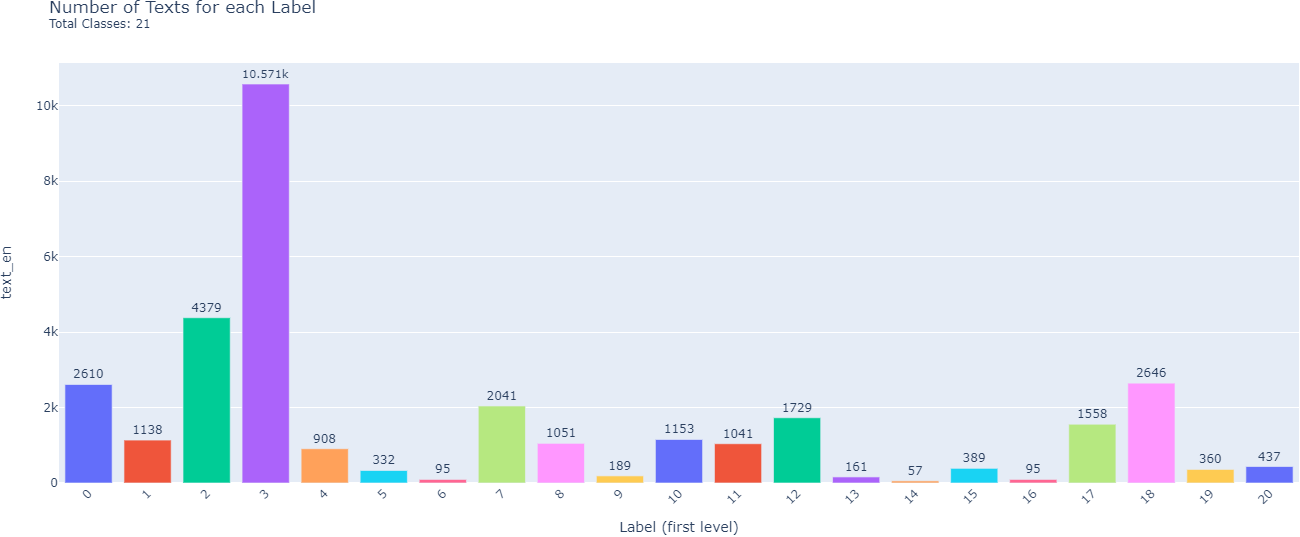
\includegraphics[width=\textwidth]{data_original_classes.png}
  \caption{MultiEURLEX Dataset - Distribution of Classes and Texts Occurrences}
  \label{fig:original_classes}
\end{figure}


A preliminary analysis of the data, however, revealed that each law averaged around 1000 words, with slight fluctuations depending on the considered language. Being aware that this factor would be computationally burdensome during the training phase of the models, it was decided to choose 2000 random laws from the three classes with the most observations, i.e. class 2, 3 and 18.

Ultimately, the final dataset consists of 6000 laws, officially translated into 5 languages and belonging to 3 distinct classes.

%%%%%%%%%%%%%%%%%
% ARCHITECTURES %
%%%%%%%%%%%%%%%%%
\newpage
\section{Architectures}
\label{sec:architectures}

In order to test the impact of different languages, various architectures were chosen, belonging both to the world of neural networks and statistics. They are presented below.

\subsection{Long Short Term Memory}

The Long Short Term Memory (LSTM) is a kind of Recurrent Neural Network (RNN). RNNs are a type of networks particularly suited to the use of sequential data, or time series. 

A distinguishing characteristic from the traditional neural networks is their capacity to have a \textit{memory}: they use information obtained from previous inputs to modify their behaviour on the current input and output. They keep the information of the former inputs in memory for an unspecified time, which depends on the weight of the network nodes and the specific data. Recurrent Neural Networks do not assume that input and output are independent, as traditional networks do, but make their output depend on the previous elements in the sequence.

Figure \ref{figure:fnn_vs_rnn} shows the typical structure of a Feedforward Neural Network on the left, and that of a Recurrent Neural Network on the right.

\vspace{0.25cm}
\begin{figure}[H]
  \centering
  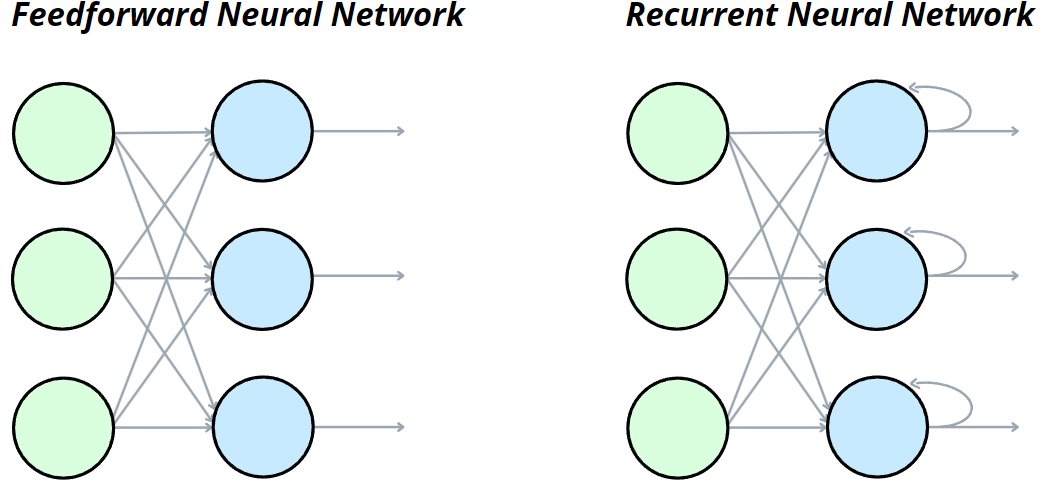
\includegraphics[width=9.5cm]{feedforward_vs_recurrent_nn.png}
  \caption{Structure of Feedforward and Recurrent Neural Networks}
  \label{figure:fnn_vs_rnn}
\end{figure}

Recurrent Neural Networks use an algorithm of \textit{backpropagation through time} to determine gradients. Backpropagation is at the basis of neural networks training, making possible the fine tuning of their weights, based on the results obtained in the previous epochs. The \textit{gradient} refers to the derivative of a function that has more than one input variable; it measures the change in all the weights of the network with respect to the change error. 

During this operation, RNNs tend to encounter two types of problems, both arising from the size of the gradient:
\begin{itemize}
  \item \textit{Vanishing Gradients}
  
  In some circumstances, the gradient is very small and continues to decrease until it becomes extremely close to 0. When this happens, the model stops learning, as its weights are no longer updated.

  \item \textit{Exploding Gradients}
  
  Conversely, the gradient can become extremely large, altering the network weights unreasonably. This causes the model to become unstable and consequently underperforming.
\end{itemize}

Long Short Term Memory networks were conceived in response to the problems of vanishing and exploding gradient, proposing a possible solution to these issues \cite{LSTM_gentle_intro}. A clear description of the inner workings of LSTMs can be found in the paper by Graves et al. \cite{Graves2005FramewisePC} where it is detailed that:

\begin{quote}
  \textit{``An LSTM layer consists of a set of recurrently connected blocks, known as memory blocks. These blocks can be thought of a differentiable version of the memory chips in a digital computer. Each one contains one or more recurrently connected memory cells and three multiplicative units - the input, output and forget gates - that provide continuous analogues of write, read and reset operations for the cells.''}
\end{quote}

In order, what happens is:
\begin{enumerate}
  \item The cell input is multiplied by the activation of the input gate;
  \item The model output is multiplied by the output gate activation;
  \item Finally, the previous cell values are multiplied by the forget gate values. 
\end{enumerate}

The network is capable of interacting with its cells exclusively through the use of gates.  

LSTMs achieve remarkably high performance on major and complex tasks; these include language modelling, speech recognition and machine translation \cite{Zaremba2014RecurrentNN}.


\subsection{Convolutional Neural Network}

Convolutional Neural Networks (CNN) are one of the most renowned algorithms of Deep Learning. Under the Deep Learning category fall all those Artificial Neural Networks that have more than one layer (and are thus called multi-layer architectures).

The layers of CNNs are usually the following:

\begin{itemize}
  \item \textit{Convolutional Layer}
  \item \textit{Non-Linearity Layer}
  \item \textit{Pooling Layer}
  \item \textit{Fully Connected Layer}
\end{itemize}

The models that use Convolutional Neural Networks have shown over the years that they are able to achieve state of the art results in many Machine Learning problems. CNNs perform particularly well in image classification and computer vision tasks, but also in problems of Natural Language Processing \cite{Albawi2017UnderstandingOA}.

\subsection{Linear Support Vector Classifier}

In order to fully understand the idea behind the Linear Support Vector Classifier, it is first necessary to introduce some concepts that form its foundation.

First, let us introduce the notion of \textit{hyperplane}. Intuitively, it is possible to think of the hyperplane as something that divides space into two sides, where it is straightforward to determine in which of the two sides a point is located. An example of a hyperplane in two-dimensional space can be observed in Figure \ref{figure:hyperplane_2d}.

\begin{figure}[H]
  \centering
  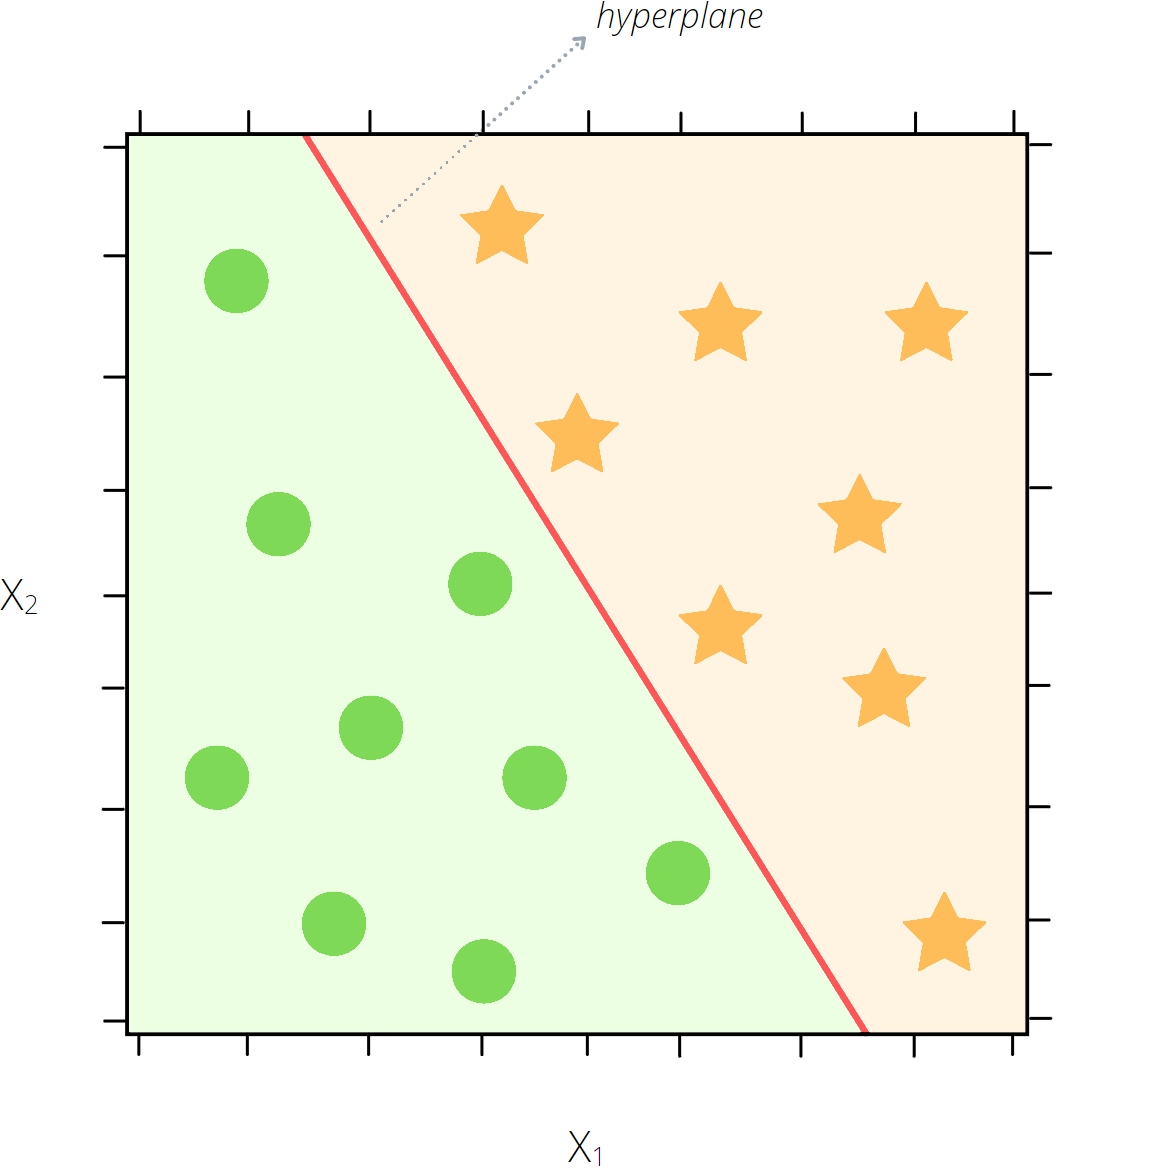
\includegraphics[width=8.5cm]{hyperplane_example.png}
  \caption{Example of Hyperplane in 2D case}
  \label{figure:hyperplane_2d}
\end{figure}

The visualisation also suggests how a hyperplane can be used to classify different observations. Let's suppose that the points in the figure represent the training set, i.e. the data initially available for training a model. It is then possible to construct a classifier in a very straightforward way: new points will be classified into \textit{green} or \textit{yellow observations} according to their position in space, given by $X_1$ and $X_2$.

Depending on how close the new observation is to the hyperplane it is also possible to have a certain degree of confidence in the correctness of the prediction. For points close to the separating hyperplane we are less certain about their class than for those further away.

There can exist an infinite number of different hyperplanes able to separate the green observations from the yellow ones. For this reason it is necessary to decide how to choose the \textit{best} hyperplane. An appropriate choice is to use the \textit{maximal margin hyperplane}, which is the hyperplane most distant from the training observations. It depends entirely on the so-called \textit{support vectors}, i.e. the points closest to it that influence its position and orientation. See Figure \ref{figure:max_margin_classifier} for an example.

\vspace{0.25cm}
\begin{figure}[H]
  \centering
  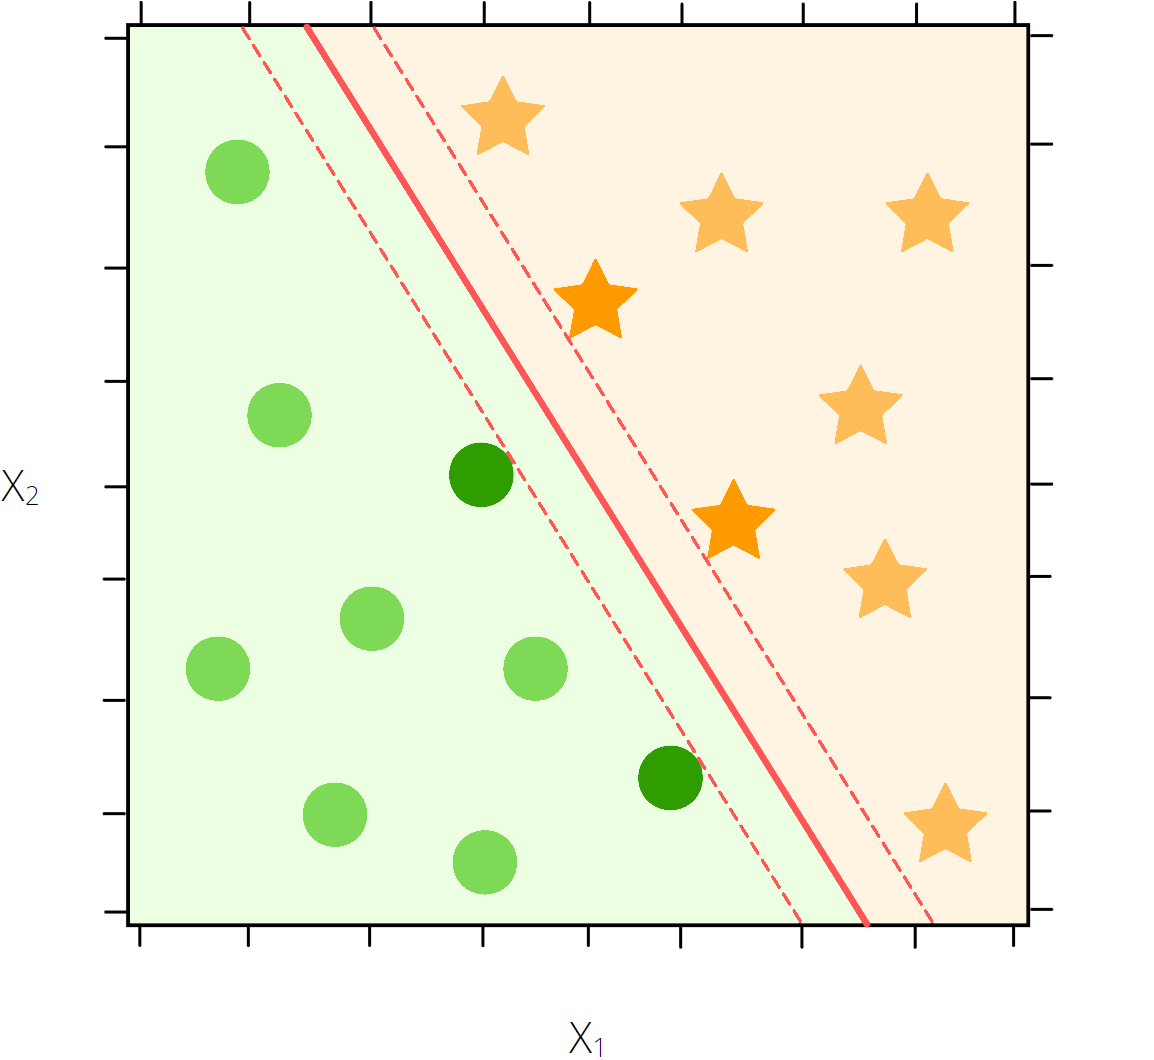
\includegraphics[width=8.5cm]{max_hyperplane.png}
  \caption{Example of Maximum Margin Hyperplane and Support Vectors (highlighted points)}
  \label{figure:max_margin_classifier}
\end{figure}

Until now we have discussed a binary case in which the two classes were linearly separable. In the event that they are not, as it happens in many real world cases, it is no longer possible to find the maximum margin hyperplane. Even if it were possible to find it, using it is not always the best solution: trying to perfectly separate the observations of the two classes makes the maximum margin hyperplane very sensitive to individual observations. It may be a better solution, in many cases, to consider a hyperplane that does not perfectly separate the training observations, but that allows to obtain a higher robustness regarding the individual observations and that correctly classifies most of the training observations.

This is indeed the objective of the support vector classifier. The model purposely allows the misclassification of certain observations, in order to correctly classify as many points as possible, while maximising the width of the margin.

Since we are not in a binary classification, we extended the binary approach to a multiclass approach using the \textit{One-VS-Rest} scheme.


%%%%%%%%%%%%%%%%%%%%%%
% EXPERIMENTAL SETUP %
%%%%%%%%%%%%%%%%%%%%%%
\newpage
\section{Experimental Setup}

\subsection{Data Cleaning and Preprocessing}

The majority of data is prone to the presence of errors and noise. This is particularly true in the field of Natural Language Processing. Therefore, textual data must be subjected to pre-processing procedures before being given to the models. 

The first critical step is data cleaning. In addition to the usual procedures such as removing duplicates, missing data, etc., when working with textual data, one often has to deal with texts that contain spelling mistakes, the use of jargon and symbols that are not useful for learning models. In our specific case, using a dataset of officially translated European laws, we do not have to worry about these issues. 

Furthermore, texts always contain \textit{stopwords}, commonly used terms that do not provide information, and which it is common practice to remove. However, these removal procedures use lists of words considered to be stopwords, but there are no universal rules. In order not to give any advantages to the most frequently used languages, such as English and German, we have decided not to remove them from the texts. Furthermore, working with recurrent neural networks, stopwords could increase the contextual sense of the networks and, contrary to what usually happens in other tasks, improve the performance of the models.

Another technique used when working with texts and natural language is to apply stemming or lemmatization procedures. These are described below.
\begin{itemize}
  \item \textit{Stemming}
  
  As can be found in the article \textit{Development of a stemming algorithm} \cite{lovins1968development}:
  \begin{quote}
    \textit{``A stemming algorithm is a computational procedure which reduces all words with the same root (or, if prefixes are left untouched, the same stem) to a common form, usually by stripping each word of its derivational and inflectional suffixes.''}
  \end{quote}
  
    \item \textit{Lemmatization}
  
  It is a procedure that removes inflectional endings and returns the base or dictionary form of a word.

  This technique ensures that similar words are reduced to the same word, which often leads to higher performance in models \cite{balakrishnan2014stemming}. 

\end{itemize}

However, the same logic of stopwords applies to \textit{stemming} and \textit{lemmatisation} procedures, which are therefore not applied to texts.

The dataset has a very high quality: it was therefore only necessary to lowercase all words, remove symbols and non-unicode characters, in order to ensure the proper functioning of future architectures.

\subsection{Feature Extraction}

Feature extraction describes the process of transforming raw data into numerical features that can be processed while retaining the information in the original dataset.

There are several ways of extracting information from data, and they change depending on the type of input that is being handled. In the context of this work, the primary focus is on the extraction of features from natural language. This can be achieved by means of several procedures, described below.

\subsubsection*{Feature Extraction for Recurrent Neural Networks}

With regard to the creation of features for the recurrent neural networks used, namely Long Short Memory and Convolutional Neural Network, we performed the following procedures:

\begin{itemize}
  \item \textit{Tokenization}
  
  Tokenization involves breaking up a raw text into smaller pieces. In our case, we break down each law text into words, the tokens. 

  \item \textit{Count Token Occurrences}
  
  We count the number of occurrences of each token (word) in our five corpuses.

  This is where we noticed the first difference between the languages: the number of different words used changes considerably, as can be seen in the Table \ref{table:tot_words_for_corpuses}. The German language, for example, uses almost three times as many words as English to describe the same laws.

  \begin{table}[H]
    \centering
    \begin{tabular}{|r|c|}
    \hline
    \multicolumn{1}{|c|}{\textbf{Language}} & \multicolumn{1}{c|}{\textbf{Different Words}} \\ \hline
    English                                 & 31454                                                            \\ \hline
    German                                  & 87084                                                            \\ \hline
    Italian                                 & 44570                                                            \\ \hline
    Polish                                  & 74691                                                            \\ \hline
    Swedish                                 & 79973                                                            \\ \hline
    \end{tabular}
    \caption{Total number of different words in each language corpus.}
    \label{table:tot_words_for_corpuses}
  \end{table}


  \item \textit{Removal of Uncommon Words}
  
  The number of different words in the texts is very high. This factor would certainly negatively affect the performance of the architectures or, at the very least, make training times extremely long. 
  
  In order to avoid these possible drawbacks, all words that did not appear in the corpus at least 100 times were removed. Table \ref{table:tot_words_for_corpuses_only_common} shows the number of words left for each language after this operation.
  
  \begin{table}[H]
    \centering
    \begin{tabular}{|r|c|}
    \hline
    \multicolumn{1}{|c|}{\textbf{Language}} & \multicolumn{1}{c|}{\textbf{Different Words}} \\ \hline
    English                                 & 3506                                                            \\ \hline
    German                                  & 4216                                                            \\ \hline
    Italian                                 & 4180                                                            \\ \hline
    Polish                                  & 5255                                                            \\ \hline
    Swedish                                 & 4010                                                            \\ \hline
    \end{tabular}
    \caption{Total number of different words in each language corpus that appears at least 100 times.}
    \label{table:tot_words_for_corpuses_only_common}
  \end{table}

  After this adjustment, the disparity between languages in the number of different words has softened, but is still present.

  \item \textit{Encoding}
  
  In this last step, we created a mapping between vocabulary and index, in order to use it in the encoding of the texts. Here, we had to set a maximum token number for each text. Since the average number of words per law is about 1000, we used this value as an upper limit.


\end{itemize}


\subsubsection*{Feature Extraction for Linear Support Vector Classifier}

\textit{TODO: scrivere questa parte dopo aver implementato Linear SVC con TF-IDF}

\subsection{Implementing the Architectures}

\subsubsection*{Long Short Term Memory}

The architecture was developed using the \verb|PyTorch| framework.

The recurrent network, described in Section \ref{sec:architectures}, was implemented with the following layers:

\begin{itemize}
  \item \textit{Embedding Layer}
  \item \textit{LSTM Layer}
  \item \textit{Linear Layer}
  \item \textit{Dropout Layer}
\end{itemize}


\textit{TODO: aggiungere visualizzazione della rete migliore}

% USA QUESTO CODICE
% input_names = ['Law Text']
% output_names = ['Law Label']
% torch.onnx.export(model, batch.text, 'rnn.onnx', input_names=input_names, output_names=output_names

\subsubsection*{Convolutional Neural Network}

This architecture, like the LSTM, was also implemented via \verb|PyTorch|.

\textit{TODO: implementare in Pytorch}

\subsubsection*{Linear Support Vector Classifier}

\textit{TODO: implementare in SKLearn}

\subsection{Training Regime}



%%%%%%%%%%%
% RESULTS %
%%%%%%%%%%%
\newpage
\section{Results}



%%%%%%%%%%%%%%
% DISCUSSION %
%%%%%%%%%%%%%%
\newpage
\section{Discussion}

\subsection{About the Results}

\textit{TODO: scrivere una volta ottenuti tutti i risultati}

\subsection{Ideas for Expanding the Project}

During the course of the project, choices were made to simplify the task and the training time required by the models. This was mainly done for reasons of limited time and means at our disposal: having only one graphics card available, certain choices proved necessary.

The following is a list of suggestions and ideas through which the project could be expanded, if we had the means to do so.

\begin{itemize}
  \item It would first be interesting to use all the texts of the laws at our disposal and repeat the experiment.
  \item Furthermore, it would also be worthwhile to consider the multi-label task and observe how the architectures behave in different languages.
  \item Having multiple GPUs avalaible, the experiment could be repeated using all 23 languages from the initial dataset.
  \item A further idea is to try applying stopword removal, lemmatization and/or stemming procedures to texts. The aim here is to see if and how the performance of the models changes and if the procedures favour the most common languages.
\end{itemize}

%%%%%%%%%%%%%%%%
% BIBLIOGRAPHY %
%%%%%%%%%%%%%%%%

% add bib to TOC
\addcontentsline{toc}{section}{Bibliography}

\newpage
\bibliographystyle{plain}
\bibliography{biblio}

%%%%%%%%%%%%%%%%%%%%%%%%%%%%%%%%%%%%%%%%%%%%%%%%%%%%%%%%%%%%%%%%%%%%%%%%%%%%%%%%%%%%%%%

\end{document}
